


\section{Luck}
\noindent It's not about the prize, it's the element of luck involved...\\
\noindent  William Cukierski, Kaggle Competition Admin \\

Previously, we detailed popular methods for prediction and outlined our new methodology that accounts for specific match ups. In this section of this paper, we address the sensitivity of the Kaggle leaderboard. While it is natural to think 2nd place almost won, we aim to answer the question how close was 20th place to winning? 

% some verbiage in here... 

We quantify luck using the idea that the 2nd place team almost won and we attempt to quantify `almost.' To this end, we examine alternate realities where a losing team in an overtime game is treated instead as a winning team. We focus only on overtime games because it seems most reasonable to think of the losing team as having won in those cases. Recall that the loss function used for loss the Kaggle competition is


\begin{equation}\label{eqn:kaggle_score}
-\sum_{i=1}^n\frac{y_ilog(p_i)+ (1-y_i)log(1-p_i)}{n},
\end{equation}
where $y_i$ is a binary variable taking value 1 when the team wins and 0 otherwise and $0 \leq p_i \leq 1$ denotes the predicted value for the team in the $i$th game. We consider how dependent the rankings of individual teams are on the characteristics of the particular loss function. To answer this question we studied a couple of possible alternate loss functions but ultimately decided to use only one. We consider the following loss function: 
 
%\begin{equation}\label{eqn:first_score_function}
%-log(1-2|.5-p_i|)
%\end{equation} 

%\begin{equation}\label{eqn:second_score_function}
%-log(1-|.5-p_i|)
%\end{equation} 

\begin{equation}\label{eqn:third_score_function}
  -\sum_{i=1}^n\frac{(1-y_i)log(1-|y_i-p_i|) +y_ilog(1-|y_i-p_i|)}{n},
\end{equation} 
where in Function \ref{eqn:third_score_function}, $y_i \in \{0,0.5,1\}$ for games where the team won, went into overtime, and loss respectively. The logic behind this function was that we felt overtime games were too close and should not be penalized as heavily as tournament games with a clear victory. Moreover, the proposed loss function uses the curious facts that $-log(1-|1-p_i|) = - log(1-p_i)$ and $log(1- | 0 - p_i | ) = - log(p_i)$ for $0 \leq p_i \leq 1$. Moreover, when $y_i=0.5$, symmetry allows us to combine the two equations to collect a single log which imposes less penalties for predictions farther away from $0.5$ while also penalizing $0.5$ none in this case. Our thinking was, if the game was close and you predict a close game you shouldn't be penalized. Figure \ref{fig:scoring_functions} is a plot of the three parts of the loss function for values $0\leq p_i \leq 1$. The third part of the loss function closes resembles an absolute value loss function for tie games. Note that nothing is special about the fact that overtime games are used. This function could be employed with equal success to compare games where the ending score of the two teams is within some threshold by properly defining the $y_i$ outcomes in the data.   

\begin{figure}[H]
\centering
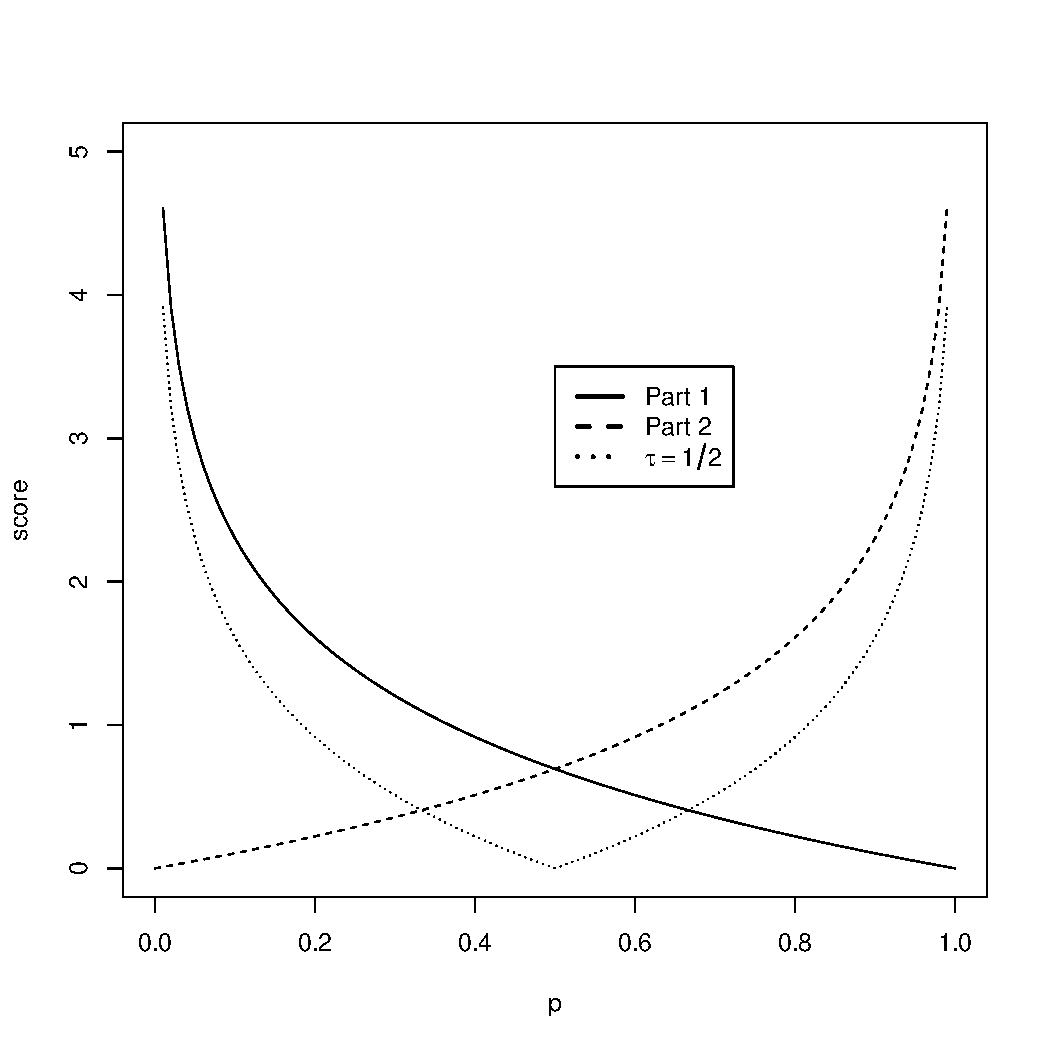
\includegraphics[width=.7\textwidth]{loss_function_plot_bw.pdf}
\caption{A plot of the three components of our proposed loss function as a function of the prediction $p_i$. We indicate part 1 and part 2 for the cases $y_i \in \{0,1\}$ respectively. }
\label{fig:scoring_functions}
\end{figure}

It is clear from looking at Figure \ref{fig:scoring_functions} that the different loss functions treat the contestant's confidence differently. Both Equations \ref{eqn:kaggle_score} and \ref{eqn:third_score_function} are symmetric about 0.5, which is aesthetically pleasing and a useful attribute for handling tied or overtime games in a slightly different manner than games with a clear victor. However, Equation \ref{eqn:kaggle_score} penalizes much more for confident predictions than Equation \ref{eqn:third_score_function}. The Kaggle competition truncated the loss functions at $10^{-15}$ and $1-10^{-15}$ for predictions of $0$ and $1$ respectively. For comparison we use the same truncation rules. Moreover, we prefer the proposed loss function because when predictions of value $0.5$ are made, no penalty is imposed. 

%  \begin{figure}[h]
%\centering
%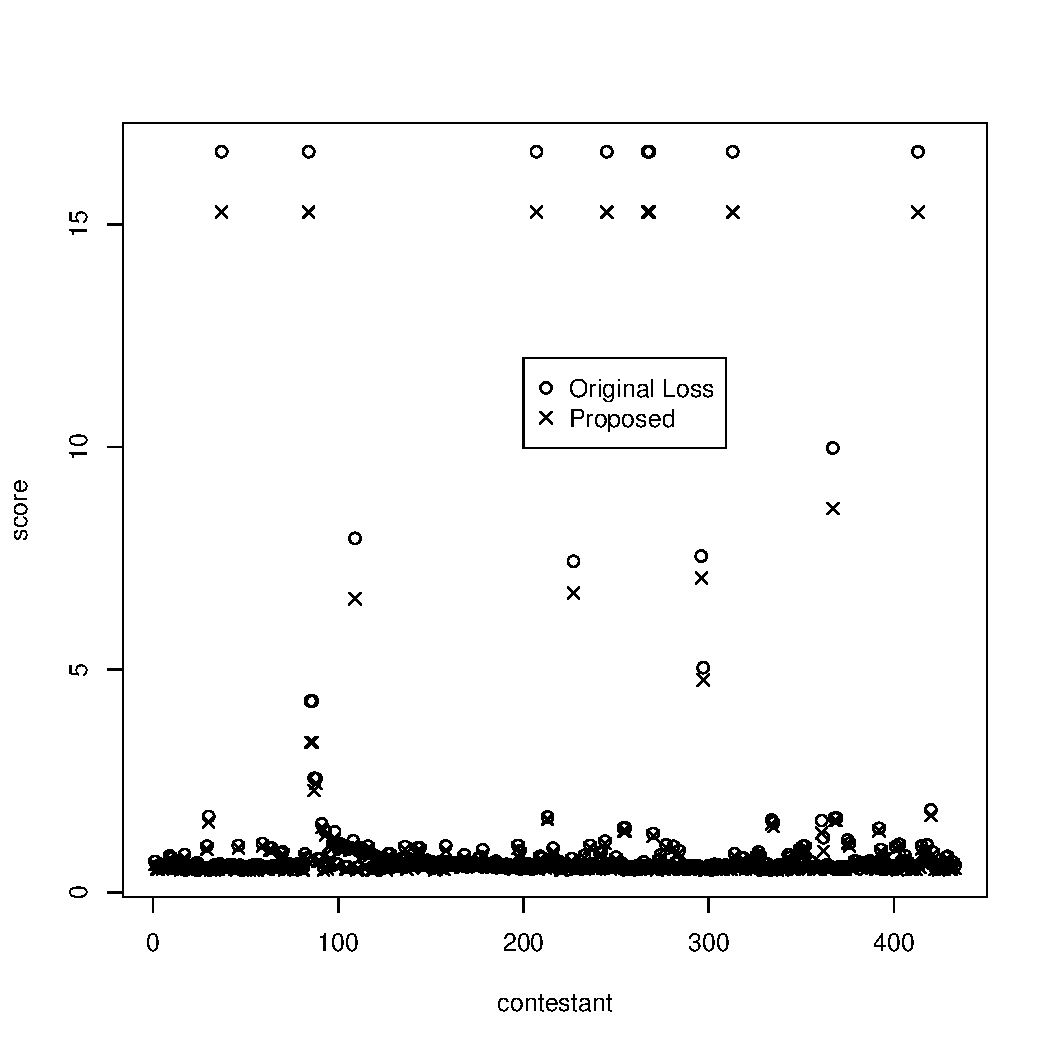
\includegraphics[width=.7\textwidth]{prelim_rank_plot1_bw.pdf}
%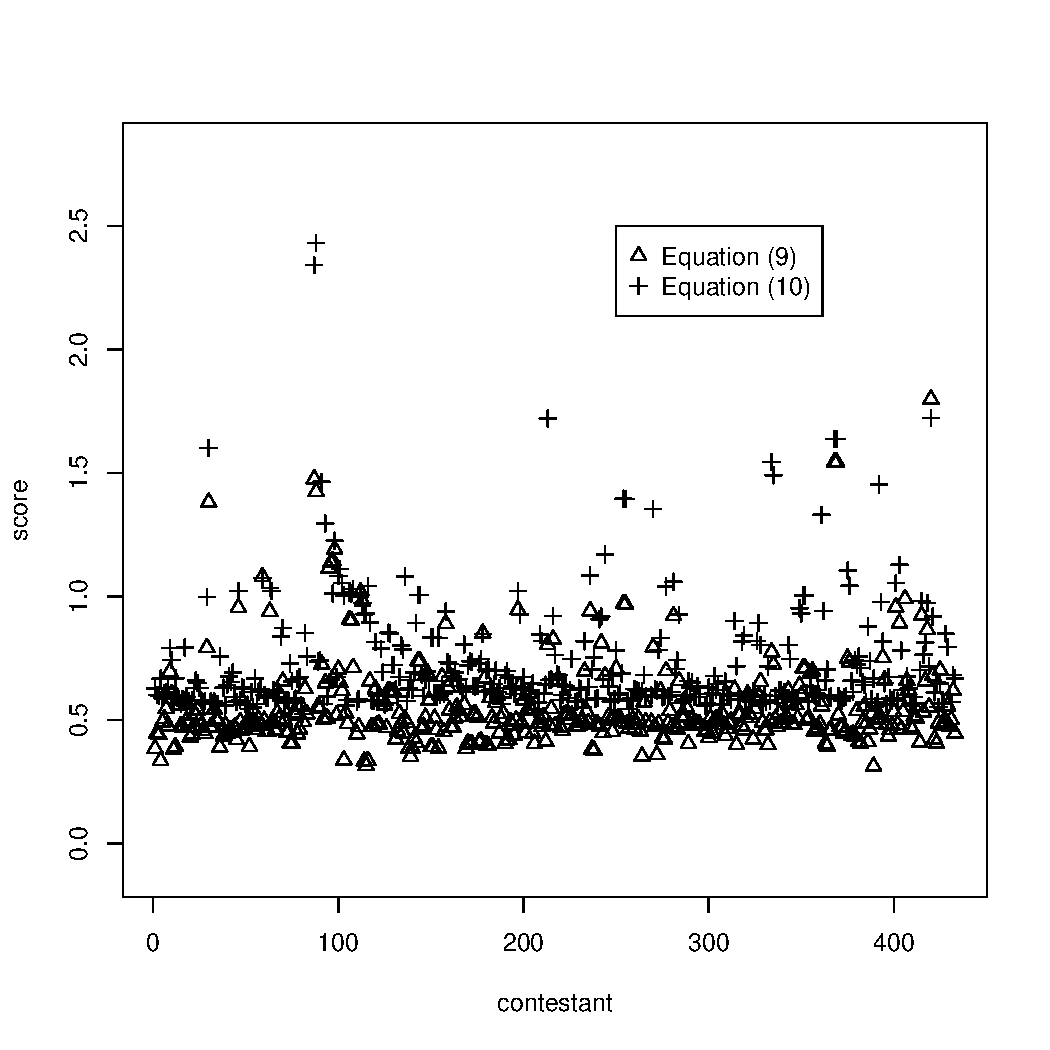
\includegraphics[width=.7\textwidth]{prelim_rank_plot2_bw.pdf}
%
%\caption{The scores of each contestant under the different loss functions. A smaller score is better.  }
%\label{fig:score_rank_plot}
%\end{figure}

Given that the choice of loss function can change the contestants' positions on the leaderboard, we did a correlation analysis of the contestant submissions resulting from the actual loss function, Equation \ref{eqn:kaggle_score} and correlated these ranks against the ranks of the contestants'  predictions under our proposed loss function, Equation \ref{eqn:third_score_function}. The results of this analysis is shown in Table \ref{tab:kendall_tau_table} beneath. There appear to be little correlation between the resultant rankings. Of course one might think, there can be little overall correlation between the rankings but still the top three might be the same or similar across the various loss functions but this turned out not to be the case. In fact, comparing the top three on the leaderboards for the two loss functions show no common contestants. Additionally, we looked at the three worst contestants as well, here the trend was the same, no common contestants when using the two criteria. 

\begin{table}[ht]
\centering
\begin{tabular}{rrr}
  \hline
Loss comparison & $\tau$ & p-value \\ 
  \hline
Equation \ref{eqn:kaggle_score} vs. Equation \ref{eqn:third_score_function} & 0.05 & 0.09 \\ 
   \hline
\end{tabular}
\label{tab:kendall_tau_table}
\caption{Kendall's $\tau$ calculation, correlation of Kaggle contestant rankings under Equation  \ref{eqn:kaggle_score} and Equation \ref{eqn:third_score_function}.}
\end{table}



Leakage is defined by \cite{schutt2013doing} as an accidental inclusion of `future' data into the training set. \cite{schutt2013doing} state that in earlier days of online comptitions they were able to consistently win competitions by systematically exploiting leakage. While much has been made in contest forums and in books  about leakage and how leakage is often exploited to win competitions, it is somewhat refreshing to see that other choices like the loss function play into the relative results of a competition. While leakage might be the result of competition administrators' errors, or a misunderstanding of the data generating process, the loss function should be chosen to match the reality of the errors made while forecasting. Nevertheless, while luck ultimately plays a role in the basketball games themselves and the results of prediction tournaments, some players are able to consistently outperform. While this section has depicted alternate outcomes that could have occurred, an actual alternate outcome will not arise until next year when the tournament occurs.  
